%% This template can be used to write a paper for
%% Computer Physics Communications using LaTeX.
%% For authors who want to write a computer program description,
%% an example Program Summary is included that only has to be
%% completed and which will give the correct layout in the
%% preprint and the journal.
%% The `elsarticle' style is used and more information on this style
%% can be found at 
%% http://www.elsevier.com/wps/find/authorsview.authors/elsarticle.
%%
%%
\documentclass[preprint,12pt]{elsarticle}

%% Use the option review to obtain double line spacing
%% \documentclass[preprint,review,12pt]{elsarticle}

%% Use the options 1p,twocolumn; 3p; 3p,twocolumn; 5p; or 5p,twocolumn
%% for a journal layout:
%% \documentclass[final,1p,times]{elsarticle}
%% \documentclass[final,1p,times,twocolumn]{elsarticle}
%% \documentclass[final,3p,times]{elsarticle}
%% \documentclass[final,3p,times,twocolumn]{elsarticle}
%% \documentclass[final,5p,times]{elsarticle}
%% \documentclass[final,5p,times,twocolumn]{elsarticle}

%% if you use PostScript figures in your article
%% use the graphics package for simple commands
%% \usepackage{graphics}
%% or use the graphicx package for more complicated commands
%% \usepackage{graphicx}
%% or use the epsfig package if you prefer to use the old commands
%% \usepackage{epsfig}

%% The amssymb package provides various useful mathematical symbols
\usepackage{amssymb}
%% The amsthm package provides extended theorem environments
%% \usepackage{amsthm}

%% The lineno packages adds line numbers. Start line numbering with
%% \begin{linenumbers}, end it with \end{linenumbers}. Or switch it on
%% for the whole article with \linenumbers after \end{frontmatter}.
%% \usepackage{lineno}

%% natbib.sty is loaded by default. However, natbib options can be
%% provided with \biboptions{...} command. Following options are
%% valid:

%%   round  -  round parentheses are used (default)
%%   square -  square brackets are used   [option]
%%   curly  -  curly braces are used      {option}
%%   angle  -  angle brackets are used    <option>
%%   semicolon  -  multiple citations separated by semi-colon
%%   colon  - same as semicolon, an earlier confusion
%%   comma  -  separated by comma
%%   numbers-  selects numerical citations
%%   super  -  numerical citations as superscripts
%%   sort   -  sorts multiple citations according to order in ref. list
%%   sort&compress   -  like sort, but also compresses numerical citations
%%   compress - compresses without sorting
%%
%% \biboptions{comma,round}

% \biboptions{}

\newcommand{\be}{\begin{equation}}
\newcommand{\ee}{\end{equation}}
\newcommand{\ba}{\begin{eqnarray}}
\newcommand{\ea}{\end{eqnarray}}

%% This list environment is used for the references in the
%% Program Summary
%%
\newcounter{bla}
\newenvironment{refnummer}{%
\list{[\arabic{bla}]}%
{\usecounter{bla}%
 \setlength{\itemindent}{0pt}%
 \setlength{\topsep}{0pt}%
 \setlength{\itemsep}{0pt}%
 \setlength{\labelsep}{2pt}%
 \setlength{\listparindent}{0pt}%
 \settowidth{\labelwidth}{[9]}%
 \setlength{\leftmargin}{\labelwidth}%
 \addtolength{\leftmargin}{\labelsep}%
 \setlength{\rightmargin}{0pt}}}
 {\endlist}

\journal{Computer Physics Communications}

\begin{document}

\begin{frontmatter}

%% Title, authors and addresses

%% use the tnoteref command within \title for footnotes;
%% use the tnotetext command for the associated footnote;
%% use the fnref command within \author or \address for footnotes;
%% use the fntext command for the associated footnote;
%% use the corref command within \author for corresponding author footnotes;
%% use the cortext command for the associated footnote;
%% use the ead command for the email address,
%% and the form \ead[url] for the home page:
%%
%% \title{Title\tnoteref{label1}}
%% \tnotetext[label1]{}
%% \author{Name\corref{cor1}\fnref{label2}}
%% \ead{email address}
%% \ead[url]{home page}
%% \fntext[label2]{}
%% \cortext[cor1]{}
%% \address{Address\fnref{label3}}
%% \fntext[label3]{}

\title{{\tt APFELgrid}: a fast interface to hadronic observables for
  fits of parton densities}

%% use optional labels to link authors explicitly to addresses:
%% \author[label1,label2]{<author name>}
%% \address[label1]{<address>}
%% \address[label2]{<address>}

\author[a]{Valerio Bertone}
\author[b]{Stefano Carrazza}
\author[a]{Nathan P. Hartland\corref{author}}

\cortext[author] {Corresponding author.\\\textit{E-mail address:} nathan.hartland@physics.ox.ac.uk}
\address[a]{Rudolf Peierls Centre for Theoretical Physics,\\ 1 Keble Road, University of Oxford, OX1 3NP, Oxford, UK}
\address[b]{TH Unit, CERN, CH-1211 Geneva 23, Switzerland}

\begin{abstract}
We present a new method conceived to ease the inclusion of hadronic
observables into parton distribution function (PDF) fits. Our
technique relies on the the same principles adopted by the existing
fast interfaces but implements a set of improvements aimed at
optimizing the performance in the context of PDF fits where many
iterations and many predictions for each iteration are usually
required. The main novelties are the precomputation of the PDF and
$\alpha_s$ evolution and the optimisation of the numerical convolution
between hard cross sections and PDFs. We demonstrate that our technique
can lead to a substantial speed improvement as compared to the
existing interfaces.
\end{abstract}

\begin{keyword}
%% keywords here, in the form: keyword \sep keyword
QCD; parton distribution functions; fast predictions.

\end{keyword}

\end{frontmatter}

\begin{small}
\noindent
{\em Manuscript Title:} {\tt APFELgrid}: a fast interface to hadronic observables for
  fits of parton densities                                      \\
{\em Authors:} V.~Bertone, S.~Carrazza, N.P.~Hartland                                               \\
{\em Program Title:} {\tt APFELgrid}                                          \\
{\em Journal Reference:}                                      \\
  %Leave blank, supplied by Elsevier.
{\em Catalogue identifier:}                                   \\
  %Leave blank, supplied by Elsevier.
{\em Licensing provisions:}                                   \\
  %enter "none" if CPC non-profit use license is sufficient.
{\em Programming language:}                                   \\
{\em Computer:}                                               \\
  %Computer(s) for which program has been designed.
{\em Operating system:}                                       \\
  %Operating system(s) for which program has been designed.
{\em RAM:} bytes                                              \\
  %RAM in bytes required to execute program with typical data.
{\em Number of processors used:}                              \\
  %If more than one processor.
{\em Supplementary material:}                                 \\
  % Fill in if necessary, otherwise leave out.
{\em Keywords:} Keyword one, Keyword two, Keyword three, etc.  \\
  % Please give some freely chosen keywords that we can use in a
  % cumulative keyword index.
{\em Classification:}                                         \\
  %Classify using CPC Program Library Subject Index, see (
  % http://cpc.cs.qub.ac.uk/subjectIndex/SUBJECT_index.html)
  %e.g. 4.4 Feynman diagrams, 5 Computer Algebra.
{\em External routines/libraries:}                            \\
  % Fill in if necessary, otherwise leave out.
{\em Subprograms used:}                                       \\
  %Fill in if necessary, otherwise leave out.
{\em Catalogue identifier of previous version:}*              \\
  %Only required for a New Version summary, otherwise leave out.
{\em Journal reference of previous version:}*                  \\
  %Only required for a New Version summary, otherwise leave out.
{\em Does the new version supersede the previous version?:}*   \\
  %Only required for a New Version summary, otherwise leave out.
{\em Nature of problem:}\\
  %Describe the nature of the problem here.
   \\
{\em Solution method:}\\
  %Describe the method solution here.
   \\
{\em Reasons for the new version:}*\\
  %Only required for a New Version summary, otherwise leave out.
   \\
{\em Summary of revisions:}*\\
  %Only required for a New Version summary, otherwise leave out.
   \\
{\em Restrictions:}\\
  %Describe any restrictions on the complexity of the problem here.
   \\
{\em Unusual features:}\\
  %Describe any unusual features of the program/problem here.
   \\
{\em Additional comments:}\\
  %Provide any additional comments here.
   \\
{\em Running time:}\\
  %Give an indication of the typical running time here.
   \\
* Items marked with an asterisk are only required for new versions
of programs previously published in the CPC Program Library.\\
\end{small}

\clearpage

\tableofcontents

%% main text
\section{Introduction}\label{sec:intro}

The need for fast and accurate cross-section predictions in the Large
Hadron Collider (LHC) era is becoming increasingly important. In fact,
the outstanding amount of precise data produced by the LHC experiments
is bound to provide a very stringent constraint on the proton parton
distribution functions (PDFs) on the condition that as many
measurements as possible are included in PDF fits with the highest
accuracy possible. However, the direct use of most of the codes that
provide predictions for non-inclusive hadron-collider observables in a
PDF fit, which typically requires a large number of iterations, is not
viable because the time required to obtain accurate predictions is
usually of the order of a few hours or more. In order to overcome this
limitation, the typical strategy adopted relies on the precomputation
of the partonic hard cross sections in such a way that the numerical
convolution with any set of PDFs can be quickly performed {\it a
  posteriori} by means of interpolation techniques.

Examples of the implementation of this strategy are {\tt
  APPLgrid}~\cite{Carli:2010rw} and {\tt
  FastNLO}~\cite{Wobisch:2011ij}. For the computation of the hard
cross sections, these packages rely on external codes to which they
are interfaced, more or less directly, by means of a suite of
functions whose scope is that of filling up PDF- and
$\alpha_s$-independent look-up tables of cross-section weights that can
subsequently be combined with an arbitrary set of PDFs. Examples of
codes that have been directly interfaced to {\tt APPLgrid} and/or to
{\tt FastNLO} are {\tt MCFM}~\cite{Campbell:2010ff} and {\tt
  NLOJet++}~\cite{Nagy:2003tz}. More recently, dedicated interfaces to
automated general-purpose Monte Carlo (MC) event generators have been
developed. In particular, the {\tt aMCfast} and {\tt MCgrid} codes
have been specifically designed to extract the relevant information
from the {\tt MadGraph5\_aMC@NLO}~\cite{Alwall:2014hca} and {\tt
  SHERPA}~\cite{Gleisberg:2008ta} event generators, respectively, and
fill up look-up interpolation tables in the {\tt APPLgrid} and/or {\tt
  FastNLO} format.

While these tools have proven to be extremely useful for the
extraction of parton densities, the great amount of experimental data
that has become available thanks to the LHC and that are or are going
to be included into the current PDF analyses is stretching the
capabilities of the general strategy as well as its
implementations. In fact, presently a typical global PDF fit includes
thousands of hadronic data points whose predictions have to be
computed thousands of times during the minimisation process. As a
consequence, the ``standard'' tools, $i.e.$ {\tt APPLgrid} and {\tt
  FastNLO}, might not be fast enough to meet the needs of the modern
PDF fitters. For this reason we believe that a high-performance tool
tailored for PDF analyses is becoming increasingly desirable.

The so-called {\tt FastKernel} method, developed in the framework of
the NNPDF global analyses~\cite{Ball:2010de}, was conceived to address
this problem. The basic principle of this method is the maximisation
of the precomputation with the consequent minimisation of the amount
of operations needed to be performed during the PDF fit. In
particular, the {\tt FastKernel} method relies on the precomputation
of the partonic hard cross sections and the DGLAP evolution kernels
and their combination into a single look-up table, which we call {\tt
  FKtable}, in such a way that the prediction for a given hadronic
observable can be obtained by a single numerical convolution between
the respective {\tt FKtable} and the initial scale PDFs, which are
the quantities that are usually fitted to data.

In this paper we present a public implementation of the {\tt
  FastKernel} method in which the partonic hard cross sections are
taken from any given {\tt APPLgrid} look-up table while the DGLAP
evolution kernels are provided by the {\tt APFEL}
code~\cite{Bertone:2013vaa}. We named the resulting code {\tt
  APFELgrid}.

The outline of this paper is the following. In
Sect.~\ref{sec:FastKernel} we present the tecnical details of the
implemantation of the {\tt FastKernel} method.

\section{The FastKernel method}\label{sec:FastKernel}

Hadron collider observables are typically computed in QCD by a double
convolution of parton densities with a hard scattering
cross-section. Consider for example the calculation of a general cross
section $pp\to X$ with a set of parton distribution functions $\{f\}$
up to order $N_\alpha$ in the strong coupling \be \sigma_{pp\to X} =
\sum_{p}^{N_\alpha}\left( \frac{\alpha_s(Q^2)}{2\pi}
\right)^{p+p_{\mathrm{LO}}} \int dx_1\, dx_2\, f_i(x_1,Q^2)\;
d\hat{\sigma}_{ij\to X}\; f_j(x_2,Q^2) \, \label{eq:hadconv} \ee where
$p_{\mathrm{LO}}$ is the leading order power of the strong coupling
for the process $pp\to X$, $Q^2$ is the hard scale of the process and
the indices $i,j$ sum over the active partonic species in the
calculation. The central observation of tools such as {\tt APPLgrid}
and {\tt FastNLO} is that such a calculation can be expressed as a
more computationally efficient product \be
\label{eq:applconv}
\sigma = \sum_p \sum_{s}^{N_{\mathrm{sub}}} \sum_{\alpha,\beta}^{N_x} \sum_{\tau}^{N_{Q}}
W_{\alpha\beta\tau}^{(p)(s)} \, \left( \frac{\alpha_s\left(Q^2_{\tau}\right)}{2\pi}\right)^{p}
F^{(s)}\left(x_{\alpha}, x_{\beta},  Q^2_{\tau}\right),
\ee
in terms of a precomputed set of coefficients $W$ obtained by convolving the hard scattering cross-section with a set of interpolating functions in the scale of the process and the parton-$x$ of each incoming parton. In Eqn. \ref{eq:applconv} the indices $\alpha, \beta$ run over points in the $x$-space interpolation grid, $\tau$ runs over the factorisation/renormalisation scale and $s$ runs over the (process-specific) parton subprocess densities defined as
\be F^{(s)}\left(x_{\alpha}, x_{\beta},  Q^2_{\tau}\right) =  \sum_{i,j}^{13} C^{(s)}_{ij}  \left( f_i(x_{\alpha},Q^2_\tau)f_j(x_{\beta},Q^2_\tau) \right).  \label{eq:APPLsubproc}\ee
Additionally a number of tools (e.g {\tt APFEL}, {\tt HOPPET}) are available which perform PDF evolution via an analogous procedure. PDFs at some scale $Q^2_\tau$ evaluated upon an interpolation grid can be calculated from a set of PDFs at some initial scale $Q^2_0$ as
\be
f_i(x_{\alpha},Q^2_\tau) = \sum_{k}^{n_f} \sum_\beta^{N_x} A^\tau_{\alpha\beta ik}\; f_k(x_\beta,Q^2_0). \label{eq:fastPDFfinal_recalled}
\ee 
where the table $A$ interpolates DGLAP evolution kernels upon an interpolation grid in $x$. Given these interpolated coefficients, we may replace the (general-scale) PDFs used in the subprocess parton density Eqn. \ref{eq:APPLsubproc} with their equivalent expressions c.f Eqn. \ref{eq:fastPDFfinal_recalled} like so
\ba F^{(s)}\left(x_{\alpha}, x_{\beta},  Q^2_{\tau}\right) &=&  \sum_{i,j}^{13} \sum_{k,l}^{n_f}  \sum_{\delta,\gamma}^{N_x} C^{(s)}_{ij}  \left[  A^\tau_{\alpha\delta ik}\; f_k(x_\delta,Q^2_0) A^\tau_{\beta\gamma jl}\; f_l(x_\gamma,Q^2_0) \right]\;\;\; \\
&=&   \sum_{k,l}^{n_f}\sum_{\delta,\gamma}^{N_x} \widetilde{C}^{(s),\tau}_{kl,\alpha\beta\gamma\delta} f_k(x_\delta,Q^2_0) f_l(x_\gamma,Q^2_0), \label{eq:FK1}
\ea
where the object
\be \widetilde{C}^{(s),\tau}_{kl,\alpha\beta\gamma\delta} = \sum_{i,j}^{13} C^{(s)}_{ij} A^\tau_{\alpha\delta ik} A^\tau_{\beta\gamma jl}.\ee
combines the operations of subprocess density construction and PDF evolution. Going further it is possible to then use the expression for subprocess parton densities in Eqn.~\ref{eq:FK1} in the full cross-section calculation:
\be
\sigma = \sum_p \sum_{s}^{N_{\mathrm{sub}}} \sum_{\alpha,\beta}^{N_x^\prime} \sum_{\tau}^{N_{Q}}
W_{\alpha\beta\tau}^{(p)(s)} \, \left( \frac{\alpha_s\left(Q^2_{\tau}\right)}{2\pi}\right)^{p}
 \sum_{k,l}^{n_f}\sum_{\delta,\gamma}^{N_x} \widetilde{C}^{(s),\tau}_{kl,\alpha\beta\gamma\delta} f_k(x_\delta,Q^2_0) f_l(x_\gamma,Q^2_0).
\ee
Performing some further contractions it is possible to obtain an extremely compact expression for the calculation of the cross-section in question, in terms of only the initial-scale PDFs and summing only over the initial scale interpolating $x$-grid and incoming parton flavors.
\be
\label{eq:FK}
\sigma = \sum_{k,l}^{n_f}\sum_{\delta,\gamma}^{N_x} 
\widetilde{W}_{kl\delta\gamma} \,f_k(x_\delta,Q^2_0) f_l(x_\gamma,Q^2_0),
\ee
where the object
\be
\label{eq:FKTable}
\widetilde{W}_{kl\delta\gamma} = \sum_p \sum_{s}^{N_{\mathrm{sub}}} \sum_{\alpha,\beta}^{N_x^\prime} \sum_{\tau}^{N_{Q}}
W_{\alpha\beta\tau}^{(p)(s)} \, \left( \frac{\alpha_s\left(Q^2_{\tau}\right)}{2\pi}\right)^{p}\widetilde{C}^{(s),\tau}_{kl,\alpha\beta\gamma\delta} .
\ee
is referred to here as an {\tt FK} table, and combines the information stored in {\tt APPLgrid}-style interpolated weight grids with analogously interpolated DGLAP evolution kernels. Such a combination
enables for a maximally computationally-efficient expression for the calculation of observables at hadron colliders.

\section{{\tt APFELgrid} manual}

\section{Benchmark}

In this section we discuss...

%%%%%%%%%%%%%%%%%%%%%%%%%%%%%%%%%%%%%%%%%%%%%%%%%%%%%%%%%%
\begin{figure}[h]
\centering
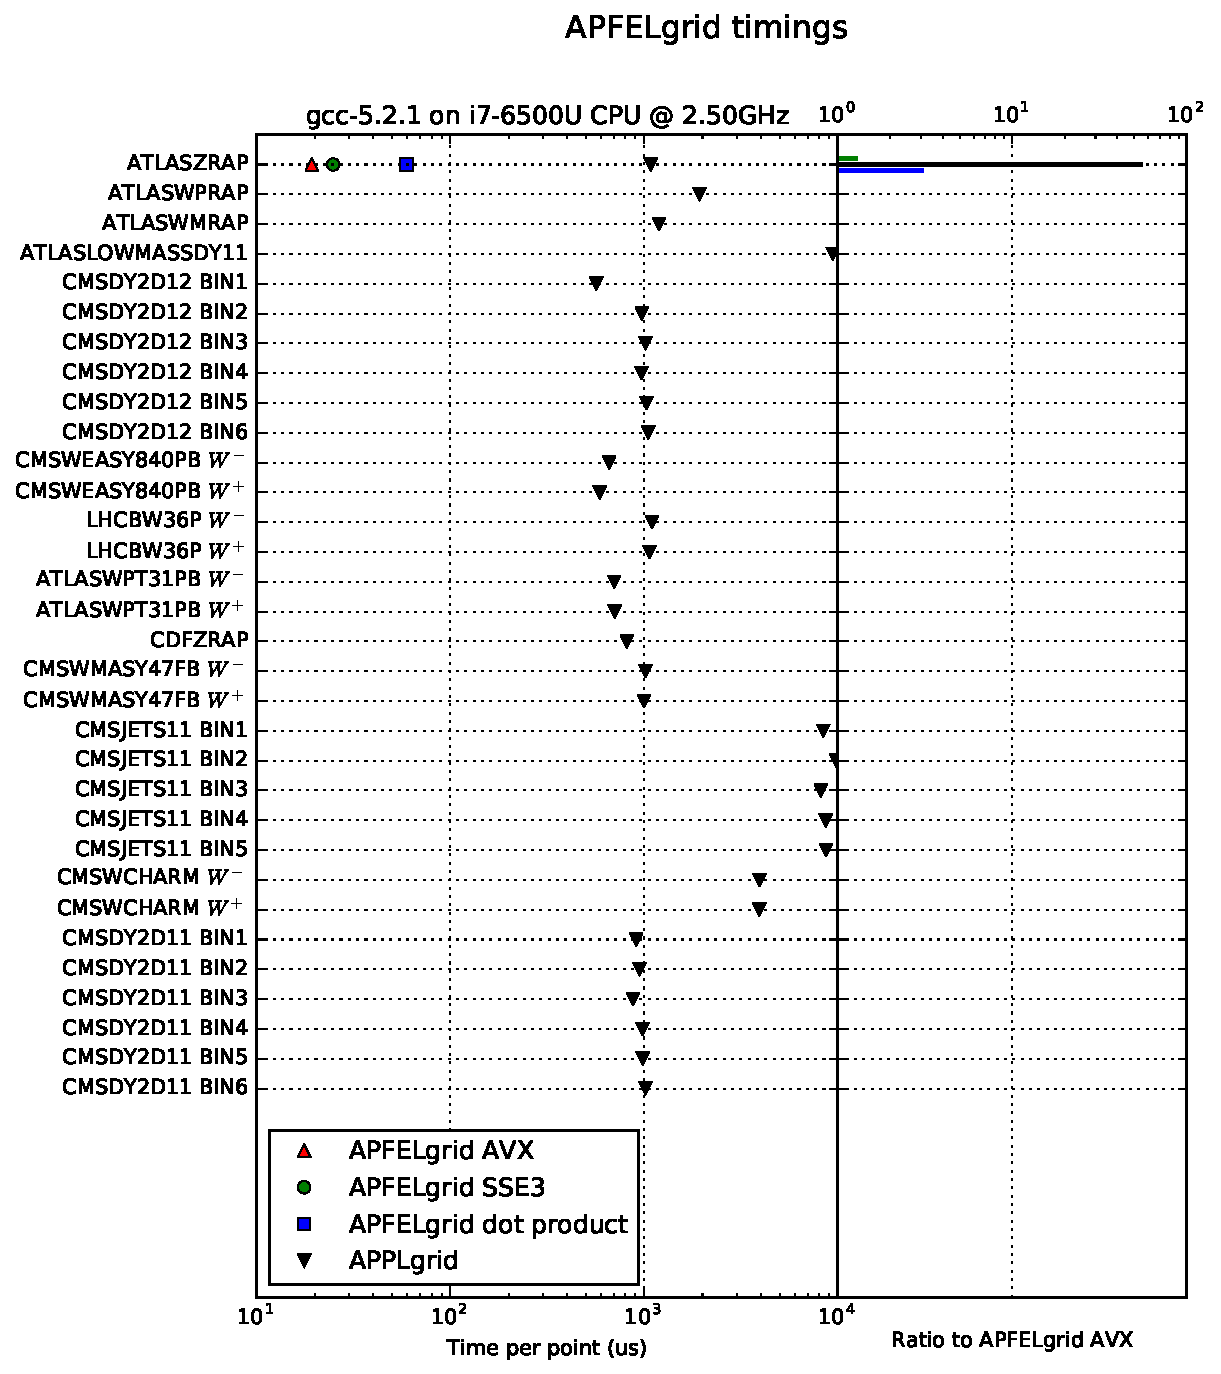
\includegraphics[scale=0.4]{plots/t0}
\caption{\small Performance comparisons between {\tt APFELgrid} with
  AVX, SSE3 and double precision convolution and {\tt APPLgrid}
  convolution time per point and process.}
\label{fig:benchmark}
\end{figure}
%%%%%%%%%%%%%%%%%%%%%%%%%%%%%%%%



%% The Appendices part is started with the command \appendix;
%% appendix sections are then done as normal sections
%% \appendix

%% \section{}
%% \label{}

%% References
%%
%% Following citation commands can be used in the body text:
%% Usage of \cite is as follows:
%%   \cite{key}         ==>>  [#]
%%   \cite[chap. 2]{key} ==>> [#, chap. 2]
%%

%% References with bibTeX database:

\bibliographystyle{elsarticle-num}
\bibliography{paper.bib}

%% Authors are advised to submit their bibtex database files. They are
%% requested to list a bibtex style file in the manuscript if they do
%% not want to use elsarticle-num.bst.

%% References without bibTeX database:

% \begin{thebibliography}{00}

%% \bibitem must have the following form:
%%   \bibitem{key}...
%%

% \bibitem{}

% \end{thebibliography}

\end{document}

%%
%% End of file 
